\documentclass[aspectratio=169]{beamer}
\usepackage[T1]{fontenc}
\usepackage[utf8]{inputenc}
\usepackage{listings}
\usepackage{xcolor}
\usepackage{hyperref}
\usepackage{graphicx}
\usepackage{textcomp}
\usepackage{tikz}
\usepackage{tcolorbox}
\usepackage{menukeys}
\usepackage{pdfpages}

\tcbuselibrary{listings}

\usefonttheme[onlymath]{serif}

\usecolortheme[RGB={37,68,113}]{structure}
\usetheme{Dresden}

% generic colors
\definecolor{dirblue}{HTML}{9bc1ff}

% TheAlternative colors
\definecolor{ldorange}{HTML}{F18A20}
\definecolor{ldblue}{HTML}{254471}

%Apply TheAlt colors to theme
\setbeamercolor{section in head/foot}{fg=ldorange}
\setbeamercolor{author in head/foot}{fg=white}
\setbeamercolor{subsection in head/foot}{fg=white}
\setbeamercolor{caption name}{fg=vlg}
\setbeamercolor{caption}{fg=vlg}
\setbeamercolor{frametitle}{fg=ldblue}
\setbeamercolor{title}{fg=ldorange}
\setbeamercolor{institute}{fg=ldblue}
\setbeamertemplate{itemize item}[circle]
\setbeamercolor{itemize item}{fg=ldorange}

% make including pdfs work
\setbeamercolor{background canvas}{bg=}

\setbeamerfont{title}{series=\bfseries}

\setbeamertemplate{caption}{\raggedright\insertcaption\par}
\setbeamertemplate{navigation symbols}{}
\setbeamertemplate{bibliography item}[text]

% white-on-black lstlisting env with rounded corners
\newenvironment{bashenv}[1][\small]{%
    \tcblisting{listing only,colback=black,colframe=black,
        enlarge top by=0mm,left=-0mm,top=-2mm,bottom=-2mm,
        listing options={language=bash,
            escapechar=§,
            basicstyle=#1\color{white}\ttfamily,
            backgroundcolor=\color{black},
            breaklines=true,
            keepspaces=true,
            showstringspaces=false,
            columns=fullflexible}}}
{\endtcblisting}

% mark a spot for e.g. drawing an arrow to it
\newcommand\tikzmark[1]{\tikz[remember picture,overlay]\node[inner xsep=0pt](#1){};}

% \newcommand\Warning{%
%     \makebox[1.4em][c]{\raisebox{-0.45em}{%
%         \makebox[0pt][c]{\raisebox{0.25em}{\large!}}%
%         \makebox[0pt][c]{\color{red}\Huge$\bigtriangleup$}}}%
%         \hspace{0.7em}%
% }

% a red warning box
\definecolor{lred}{HTML}{ffd6dd}
\newtcolorbox{WarningBox}{%
    colframe=red,
    colback=lred}



\title{The Console Toolkit}
\author{Lukas Tobler}
\institute{TheAlternative, SSC | ETHZ and UZH}
\date{HS 2018}

\begin{document}
	\begin{frame}
		\titlepage%
	\end{frame}

    \section{Introduction}

    \begin{frame}[t,fragile]{Why the console? It's already current year!}
        \begin{itemize}
            \item People ask for it
            \item Still an excellent interface for complex tasks
            \item Many advanced tools only available on the command line
            \item Can be much faster than GUI tools
            \item Allows easy remote access to other computers
            \item Skills portable to every Unix-like system
        \end{itemize}
    \end{frame}

    \begin{frame}[t,fragile]{Course outline}
        \begin{columns}
            \column{0.5\textwidth}
            \textbf{Part 1}
            \column{0.5\textwidth}
            \textbf{Part 2}
        \end{columns}
    \end{frame}

    \begin{frame}[t,fragile]{What is the console}
        \begin{columns}[T]
            \column{0.4\textwidth}
            \begin{itemize}
                \item Keyboard-only interface to your computer
                \item Related terms: \emph{console}, \emph{terminal},
                    \emph{shell}, \emph{bash}, \emph{command prompt},
                    \emph{command line interface}
            \end{itemize}
            \column{0.6\textwidth}
            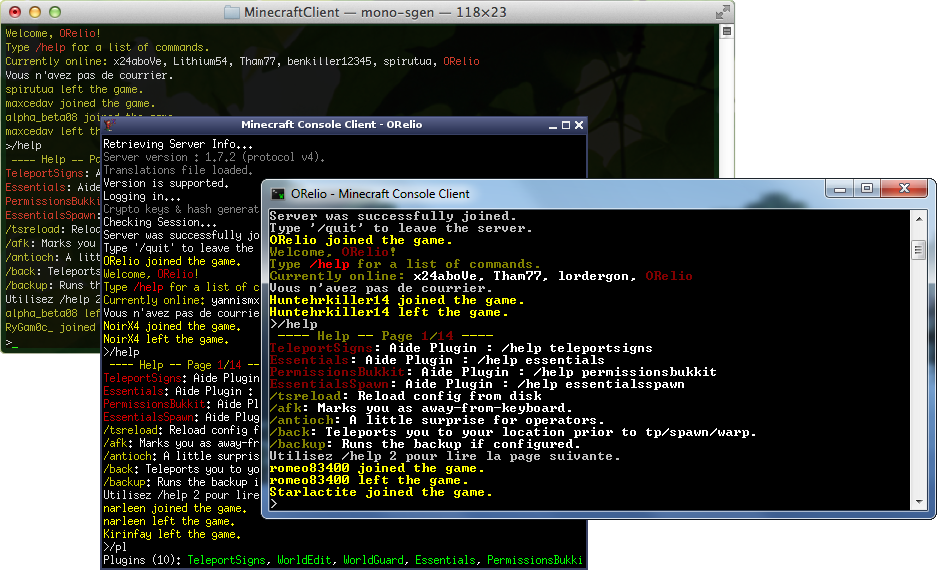
\includegraphics[width=\columnwidth]{img/consoles.png}
        \end{columns}
    \end{frame}

    \section{File system navigation}

    \begin{frame}[t,fragile]{The 70s were interesting times, or so I'm told}
        \textbf{Unix dogma: \emph{Everything is a file!}} \\
        \begin{itemize}
            \item Data files
            \item Directories (or ``folders'')
            \item Storage devices
            \item Keyboards
            \item Printers
            \item Cameras
            \item \emph{But not network sockets \ldots}
        \end{itemize}
    \end{frame}

    \begin{frame}[t,fragile]{File system}
        \begin{columns}[T]
            \column{0.5\textwidth}
            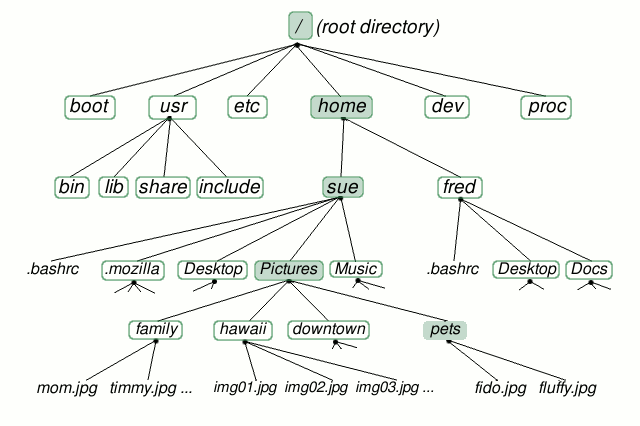
\includegraphics[width=\columnwidth]{img/dirtree.png}
            \column{0.5\textwidth}
            \begin{itemize}
                \item File system organized as tree
                \item Everything under \texttt{/}, the root directory
                \item In the console, you will be at some point in the tree,
                    the \emph{working directory}
            \end{itemize}
        \end{columns}
    \end{frame}

    \begin{frame}[t,fragile]{Working directory}
        \begin{columns}[T]
            \column{0.5\textwidth}
            \begin{itemize}
                \item Where am I? \textrightarrow \: \texttt{pwd}
                \item \underline{P}resent \underline{w}orking \underline{d}irectory
                \item Also sometimes directly shown in the prompt
                \item The tilde \texttt{\textasciitilde} means:
                    \emph{this user's home directory} (abbreviation)
            \end{itemize}
            \column{0.5\textwidth}
            \begin{bashcmd}
[luke@host ~]$ pwd
/home/luke
[luke@host ~]$
            \end{bashcmd}
        \end{columns}
    \end{frame}

    \begin{frame}[t,fragile]{Listing files}
        \begin{columns}[T]
            \column{0.5\textwidth}
            \begin{itemize}
                \item What is in here? \textrightarrow \: \texttt{ls}
                \item ``list''
            \end{itemize}
            \column{0.5\textwidth}
            \begin{bashcmd}
[luke@host ~]$ ls
§\textcolor{dirblue}{Desktop}§
§\textcolor{dirblue}{Documents}§
§\textcolor{dirblue}{Downloads}§
§\textcolor{dirblue}{Music}§
§\textcolor{dirblue}{Pictures}§
§\textcolor{dirblue}{Videos}§
cat1.jpg
cat2.jpg
[luke@host ~]$
            \end{bashcmd}
        \end{columns}
    \end{frame}

    \section{Meta}

    \begin{frame}[t,fragile]{Go somewhere else}
        \begin{columns}[T]
            \column{0.5\textwidth}
            \begin{itemize}
                \item I want to go to some other directory! \textrightarrow \: \texttt{cd}
                \item ``Change directory''
                \item Absolute path: Whole path from the root, like:
                    \texttt{/home/luke/pictures/cat1.png}
                \item Relative path: Path relative to the current working
                    directory, like \texttt{pictures/cat1.png}
            \end{itemize}
            \column{0.5\textwidth}
            \begin{bashcmd}
[luke@host ~]$ cd
[luke@host ~]$ pwd
/home/luke
[luke@host ~]$ cd /sys
[luke@host sys]$ pwd
/sys
[luke@host sys]$ cd ~
[luke@host ~]$ pwd
/home/luke
[luke@host ~]$ cd pictures/
[luke@host pictures]$ pwd
/home/luke/pictures
            \end{bashcmd}
        \end{columns}
    \end{frame}

    \begin{frame}[t,fragile]{Commands \& arguments}
        \vspace{0.5cm}
        \texttt{\tikzmark{a}{l}s \tikzmark{b}{-}a
            \tikzmark{c}{-}-human-readable \tikzmark{d}{/}home/luke/pictures}\\
        \begin{tikzpicture}[remember picture,overlay]
            \node[align=left,xshift=0.4cm,yshift=-1.0cm,rounded corners,
            fill=red!20,draw=red!70!black] (b1)
            {\footnotesize{command}};
            \draw[red!70!black,->] (b1) edge ([yshift=-0.05cm,xshift=7.0pt]a.south);

            \node[align=left,xshift=3.0cm,yshift=-2.3cm,rounded corners,
            fill=green!20,draw=green!70!black] (b2)
            {\footnotesize{single letter option}};
            \draw[green!70!black,->] (b2) edge ([yshift=-0.05cm,xshift=9.5pt]b.south);

            \node[align=left,xshift=3.7cm,yshift=-0.7cm,rounded corners,
            fill=green!20,draw=green!70!black] (b3)
            {\footnotesize{long option}};
            \draw[green!70!black,->] (b3) edge ([yshift=-0.05cm,xshift=1.5cm]c.south);

            \node[align=left,xshift=6.7cm,yshift=-0.7cm,rounded corners,
            fill=orange!40,draw=orange!70!black] (b4)
            {\footnotesize{arguments}};
            \draw[orange!70!black,->] (b4) edge ([yshift=-0.05cm,xshift=1.7cm]d.south);

        \end{tikzpicture}
    \end{frame}

    \begin{frame}[t,fragile]{Getting help}
        \begin{itemize}
            \item Where can I find out what options are available?
            \item Manual pages!
            \item \texttt{man}
            \item E.g.: \texttt{man ls}
        \end{itemize}
    \end{frame}

    \begin{frame}[t,fragile]{}
        \begin{bashcmd}
LS(1)                      User Commands                     LS(1)

NAME
       ls - list directory contents

SYNOPSIS
       ls [OPTION]... [FILE]...

DESCRIPTION
       List information about the FILEs (the current directory by
       default). Sort entries alphabetically if none of -cftuvSUX
       nor --sort is specified.

       Mandatory arguments to long options are mandatory for short
       options too.
                \end{bashcmd}
    \end{frame}

    \begin{frame}[t,fragile]{}
                \begin{bashcmd}
       -a, --all
              do not ignore entries starting with .

       -A, --almost-all
              do not list implied . and ..

       --author
              with -l, print the author of each file

       -b, --escape
              print C-style escapes for nongraphic characters

       --block-size=SIZE
              with -l, scale sizes by SIZE when printing them; e.g.,
              '--block-size=M'; see SIZE format below
        \end{bashcmd}
    \end{frame}

    \begin{frame}[t,fragile]{Tab completion}
        \begin{itemize}
            \item Hit \keys{\tab} to automatically complete a word you are typing
                (Command, file, ...)
            \item Hit \keys{\tab} twice to show all possible options
            \item Extremely useful terminal feature! Use always!
        \end{itemize}
    \end{frame}

    \begin{frame}[t,fragile]{Command History}
        \begin{itemize}
            \item Scroll up in your command history by pressing the
                \keys{\arrowkeyup} key
            \item Press \keys{\ctrl} + \keys{r} to search the history
        \end{itemize}
    \end{frame}

    \section{Text files}

    \begin{frame}[t,fragile]{Showing text files}
        \begin{columns}[T]
            \column{0.5\textwidth}
            \begin{itemize}
                \item Output a file's contents to the console with
                    \texttt{cat}
                \item Used to stand for ``concatenate''
            \end{itemize}
            \column{0.5\textwidth}
            \begin{bashcmd}
[luke@host ~]$ cat diary
Dear diary, today I downloaded
cat pictures from the internet.
[luke@host ~]$
            \end{bashcmd}
        \end{columns}
    \end{frame}

    \begin{frame}[t,fragile]{Reading long files}
        \begin{itemize}
            \item What if the text doesn't fit on the terminal?
            \item Use the \texttt{less} file browser
            \item Scroll up and down with \keys{\arrowkeyup}, \keys{\arrowkeydown}
            \item Exit with \keys{q}
        \end{itemize}
    \end{frame}

    \begin{frame}[t,fragile]{Copying files}
        \begin{columns}[T]
            \column{0.5\textwidth}
                \begin{itemize}
                    \item Copy command: \texttt{cp}
                    \item Syntax: \texttt{cp source destination}
                \end{itemize}
            \column{0.5\textwidth}
            \begin{bashcmd}
[luke@host ~]$ cp diary diary_copy
[luke@host ~]$ cat diary_copy
Dear diary, today I downloaded
cat pictures from the internet.
[luke@host ~]$
            \end{bashcmd}
        \end{columns}
    \end{frame}

    \begin{frame}[t,fragile]{Moving files}
        \begin{columns}[T]
            \column{0.47\textwidth}
                \begin{itemize}
                    \item Move command: \texttt{mv}
                    \item Syntax: \texttt{mv source destination}
                    \item Useful to rename files
                \end{itemize}
            \column{0.53\textwidth}
            \begin{bashcmd}
[luke@host ~]$ mv diary secret_diary
[luke@host ~]$ cat secret_diary
Dear diary, today I downloaded
cat pictures from the internet.
[luke@host ~]$
            \end{bashcmd}
        \end{columns}
    \end{frame}

    % \begin{frame}[t,fragile]{INSERT TITLE}
    %     \begin{columns}[T]
    %         \column{0.5\textwidth}
    %         \column{0.5\textwidth}
    %     \end{columns}
    % \end{frame}

\end{document}
